\documentclass{article}
\usepackage{mystyle}
\usepackage{csquotes}

\begin{document}

\title{Design Boneyard}
\author{Sam Fok}

\maketitle

\begin{displayquote}
"Good design comes from experience.
Experience comes from bad design"
\end{displayquote}

Herein is a graveyard of old, abandoned designs. These are not be formatted or documented particularly well. They remain in whatever state they were abandoned in. In the ideal world, explanations for why a design doesn't work would be particularly helpful. However, with deadlines always looming, there is little time for creating such explanations.

\section{Old Arbiter ($ARB$)}

The arbiter cell ARB sequences requests from rows or columns by arbitrating between concurrent requests. 
Each ARB instance handles requests from two children and sends requests to its parent. 
To arbitrate between $N$ children, we use $N-1$ ARB cells arranged in a binary tree.
ARB is designed to be greedy but fair.
ARB's CHP is derived from

\begin{csp}
ARB\equiv*[[#{L`1}->R;L`1;L`1;R
          \|#{L`2}->R;L`2;L`2;R]]
\end{csp}

where

\begin{tabular}[c]{rl}
$L_1$ & communicates with the first child \\
$L_2$ & communicates with the second child \\
$R$ & communicates with the parent arbiter \\
\end{tabular}

The arbitration operator can be broken out into its own process

\begin{csp}
ARB\equiv\! *[[#{L`1}->A`1;R;L`1;L`1;R;A`1]]
      \pll*[[#{L`2}->A`2;R;L`2;L`2;R;A`2]]
      \pll*[[#{A`1}->A`1;A`1\|#{A`2}->A`2;A2]]
\end{csp}

The 2-way arbiter has ports:

\begin{tabular}[]{rll}
  \code{R} & (active) & transmits request to parent \\
  \code{L1} & (passive) & receives requests from left child 1 \\
  \code{A1} & (local) & request 1 to internal arbitration circuit \\
  \code{R1} & (local) & or'ed with \code{R2} to produce \code{R} \\
  \code{L2} & (passive) & receives requests from left child 2 \\
  \code{A2} & (local) & request 2 to internal arbitration circuit \\
  \code{R2} & (local) & or'ed with \code{R2} to produce \code{R} \\
\end{tabular} \\ \\

The existing HSE for the arbiter cell is given by

\begin{hse}
*[[l1i&~ri];a1o+;r1o+;[ri&a1i];l1o+;
  [~l1i];a1o-;r1o-;[~a1i];l1o-]

*[[l2i&~ri];a2o+;r2o+;[ri&a2i];l2o+;
  [~l2i];a2o-;r2o-;[~a2i];l2o-]
\end{hse}

In words, for the process communicating with the first child,

\begin{tabular}[]{rl}
  \code{[l1i$\land$~ri]} & wait for a child's request and to not already have the parent's go-ahead \\
  \code{a1o$\uparrow$} & request permission from the arbiter circuit \\
  \code{r1o$\uparrow$} & request permission from the parent \\
  \code{[ri$\land$a1i]} & wait for permission from the parent and arbiter circuit \\
  \code{l1o$\uparrow$} & signal child to go-ahead \\
  \code{[$\neg$l1i]} & wait for child to finish \\
  \code{a1o$\downarrow$} & withdraw request from the arbiter circuit \\
  \code{r1o$\downarrow$} & withdraw request from the parent \\
  \code{[$\neg$a1i]} & wait for arbiter circuit to withdraw go-ahead permission \\
  \code{l1o$\downarrow$} & reset child go-ahead signal \\
\end{tabular} \\ \\

The process communicating with the second child has the equivalent semantics.
The initial \code{$\neg$ri} guard ensures fairness of the arbiter cell.
The existing PRS is given by

\begin{prs2}
l1i & _ri -> _a1o-
~l1i -> _a1o+

a1o & _a2i -> _a1i-
~a1o | ~_a2i -> _a1i+

~_a1i & ~_ri & _a2i -> l1o+
_a1i | _ri -> l1o-
\end{prs2}

\begin{prs2}
l2i & _ri -> _a2o-
~l2i -> _a2o+

a2o & _a1i -> _a2i-
~a2o | ~_a1i -> _a2i+

~_a2i & ~_ri & _a1i -> l2o+
_a2i | _ri -> l2o-
\end{prs2}

Note that the existing PRS does not respect the existing HSE. 
Namely, the \code{[$\neg$a1i]} guard is not respected.
Correct operation of the arbiter cell assumes that the reset of the filter 
from the arbiter circuit arrives before the reset from the parent cell acknowledge.
We will fix these issues in the next section.

%%%%%%%%%%%%%%%%%%%%%%%%%%%%%%%%%%%%%%%%%%%%%%%%%%%%%%%%%%%%%%%%%%%%%%%%%%%%%%%
\section{Rajit's probe evaluation circuit}
For reference.

\paragraph{CHP}

\begin{csp}
*[[#X&#E->E!\mathrm{true},X
  \|~#X&#E->E!\mathrm{false}]]
\end{csp}

implemented by

\begin{csp}
*[[#X->[E];E!\mathrm{true},X
  \|#E->E!\mathrm{false}]]
\end{csp}


\paragraph{HSE}

\begin{hse}
*[[Xi->t+;[~Xi];t-
  \|Ei->f+;[~Ei];f-]]
\pll
*[[t->[Ei];Eto+;[~Ei];Xo+;Eto-;[~t];Xo-
  []f->Efo+;[~f];Efo-]]
\end{hse}

\paragraph{PRS}

\begin{prs2}
t & _Xo & Ei -> _Eto-
~_Xo -> _Eto+

_Xo & t -> Efo-
~f -> Efo+

~_t & ~_Eto & ~Ei -> Xo+
_t & _Eto -> Xo-

Xo -> _Xo-
~Xo -> _Xo+

t -> _t-
~t -> _t+
\end{prs2}
%%%%%%%%%%%%%%%%%%%%%%%%%%%%%%%%%%%%%%%%%%%%%%%%%%%%%%%%%%%%%%%%%%%%%%%%%%%%%%%
\section{arbiter $CTRL$ with passive $S$ ports}
This was a candidate arbiter $CTRL$ design. 
Turns out to be more complicated than $CTRL$ with active $S$ ports so we abandoned it.

\paragraph{CHP}

\begin{csp}
CTRL\approx
  *[[#{C1}|#{C2}->P;S1;S1\star(S2;S2\star\!P)]
  
C_S\equiv
  *[C;A;A;C]
\end{csp}

\paragraph{HSE}

\begin{hse}
CTRL\equiv
  *[[c1i|c2i];po+;[pi];
    [s1i];s1o+;[~s1i];
    [s2i];s2o+;[~s2i];
    po-;[~pi];s1o-;s2o-]
\end{hse}

\begin{hse}
C_S\equiv
  *[co+;[ci];ao+;[ai];
    ao-;[~ai];co-;[~ci]]
\end{hse}

needs a state variable

\begin{hse}
C_S\equiv
  *[x+;co+;[ci];ao+;[ai];
    x-;ao-;[~ai];co-;[~ci]]
\end{hse}

\paragraph{PRS}

$CTRL\equiv$
\begin{prs2}
(c1i | c2i) & ~s2o -> po+
~s2i & s2o -> po-

pi & s1i -> s1o+
~pi -> s1o-

~s1i & s1o & s2i -> s2o+
~s1o -> s2o-
\end{prs2}

with active high inputs and outputs, $C\_S\equiv$
\begin{prs2}
ai | x -> _co-
~ai & ~x -> _co+

ci & x -> _ao-
~ci | ~x -> _ao+

~ci & ~ai -> x+
ai -> x-

~_co -> co+
_co -> co-

~_ao -> ao+
_ao -> ao-
\end{prs2}

with active low inputs and active high outputs, $C\_S\equiv$
\begin{prs2}
~_ai | ~_x -> co+
_ai & _x -> co-

~_ci & ~_x -> ao+
_ci | _x -> ao-

_ci & _ai -> _x-
~_ai -> _x+
\end{prs2}
\pagebreak
%%%%%%%%%%%%%%%%%%%%%%%%%%%%%%%%%%%%%%%%%%%%%%%%%%%%%%%%%%%%%%%%%%%%%%%%%%%%%%%
\section{post arbiter}

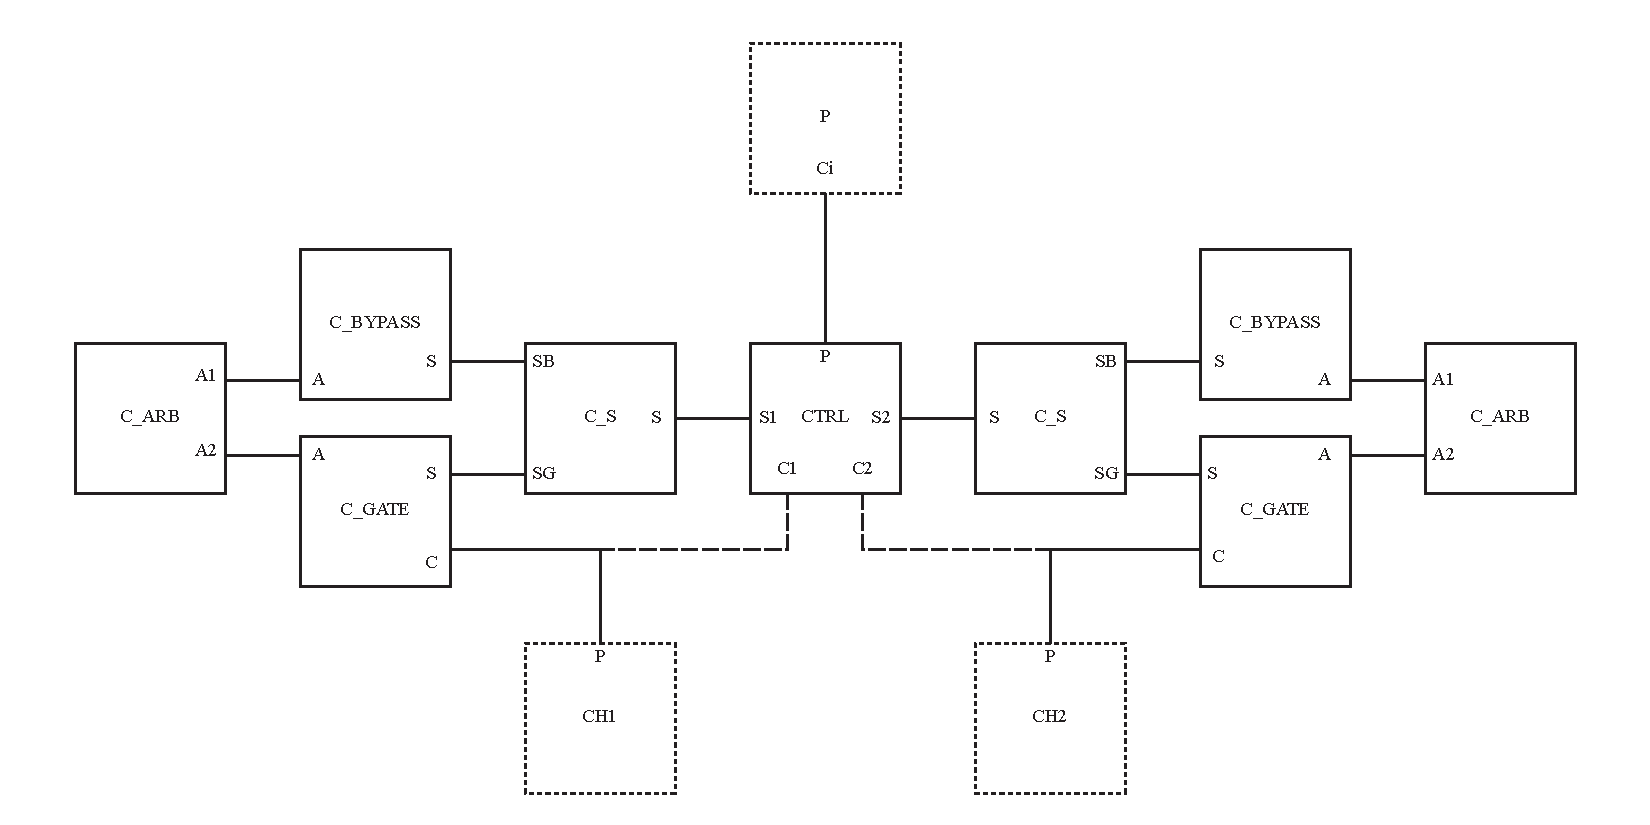
\includegraphics[width=\textwidth]{img/transmitter/arb.pdf}

\noindent CHP:

\begin{csp}
CTRL\equiv
  *[[#{C1}|#{C2}->P;S1;S1\star(S2;S2\star\!P)]]
\end{csp}
\begin{csp}
C_S\equiv
  *[(SB,SG)\star\!S;(SB,SG)\star\!S]
\end{csp}
\begin{csp}  
C_GATE\equiv
  *[C\star(A,S);C\star(A,S)]
\end{csp}
\begin{csp}
C_BYPASS\equiv
  *[S;A;S,A]
\end{csp}
\begin{csp}
C_ARB\equiv
  *[[#{A1}->A1;A1\|#{A2}->A2;A2]]
\end{csp}

\noindent HSE:

\begin{hse}
CTRL\equiv
  *[[c1i|c2i];po+;[pi];
    [s1i];s1o+;[~s1i];
    [s2i];s2o+;[~s2i];
    po-;[~pi];s1o-,s2o-]
\end{hse}
\begin{hse}
C_S\equiv
  *[[sgi|sbi];so+;[si];sgo+,sbo+;
    [~sgi&~sbi];so-;[~si];sgo-,sbo-]
\end{hse}
\begin{hse}
C_GATE\equiv    
  *[[ci];ao+,so+;[ai&si];co+;
    [~ci];ao-,so-;[~ai&~si];co-]
\end{hse}
\begin{hse}
C_BYPASS\equiv
  *[so+;[si];ao+;[ai];
    so-,ao-;[~si&~ai]]
\end{hse}
\begin{hse}
C_ARB\equiv
  *[[a1i];a1o+;[~a1i];a1o-
   \|[a2i];a2o+;[~a2i];a2o-]
\end{hse}

\noindent PRS

$CTRL\equiv$
\begin{prs2}
c1i | c2i -> po+
~s2i & s2o -> po-

pi & s1i -> s1o+
pi & ~s1i & s1o & s2i -> s2o+
~pi -> s1o-, s2o-
\end{prs2}

$C\_S\equiv$
\begin{prs}
sgi | sbi -> so+
~sgi & ~sbi -> so-

si -> sgo+, sbo+
~si -> sgo-, sbo-
\end{prs}

$C\_GATE\equiv$
\begin{prs2}
c1i -> ao+, so+
~c1i -> ao-, so-

ai & si -> c1o+
~ai & ~si -> c1o-
\end{prs2}

$C\_BY\!P\!ASS\equiv$
\begin{prs2}
~si&~ai -> so+
si -> ao+
ai -> so-, ao-
\end{prs2}

$C\_ARB\equiv$
\begin{prs2}
a1i & _a2o -> _a1o-
~a1i | ~_a2o -> _a1o+

~_a1o & _a2o -> a1o+
_a1o -> a1o-

a2i & _a1o -> _a2o-
~a2i | ~_a1o -> _a2o+

~_a2o & _a1o -> a2o+
_a2o -> a2o-
\end{prs2}
%%%%%%%%%%%%%%%%%%%%%%%%%%%%%%%%%%%%%%%%%%%%%%%%%%%%%%%%%%%%%%%%%%%%%%%%%%%%%%%
\newpage
\section{A Better Arbiter (failed. on hold)}

Starting with

\begin{csp}
ARB2\equiv*
  *[[#{L1}->R;L1;L1;R
    \|#{L2}->R;L2;L2;R]]
\end{csp}

we split out the arbitration into a separate process.

\begin{csp}
ARB2\equiv
*[[#{L1}->A1;R;L1;L1;R;A1]] \pll
*[[#{L2}->A2;R;L2;L2;R;A2]] \pll
*[[#{A1}->A1;A1\|#{A2}->A2;A2]]
\end{csp}

This arbiter is not greedy and returns the token to the parent after servicing a child.
To make it greedy yet fair, we split out communication with the parent arbiter cell into a separate process.

\begin{csp}
ARB2\equiv
  *[[#{L1}->A1;R1;L1;L1;A1;R1)]] \pll
  *[[#{L2}->A2;R2;L2;L2;A2;R2)]] \pll
  *[[#{A1}->A1;A1\|#{A2}->A2;A2]]\pll
  *[[#{R1}|#{R2}->R;
    [#{R1}->R1;R1\|~#{R1}->skip],
    [#{R2}->R2;R2\|~#{R2}->skip];
    R]]
\end{csp}

The parent communication process implements a greedy algorithm because once it acquires the token from the parent,
it will not return the token until both children have been serviced (if both have requested). 
The algorithm is fair because each child will only be serviced at most once for posession of the token.
The parent communication process can signal children processes in parallel because aribtration is handled by the arbitration process.
We use synchronizers enabled by the parent request to ensure that selection guards are mutually exclusive.


\begin{csp}
ARB2\equiv
  *[[#{L1}->A1;R1;L1;L1;A1;R1)]] \pll
  *[[#{L2}->A2;R2;L2;L2;A2;R2)]] \pll
  *[[#{A1}->A1;A1\|#{A2}->A2;A2]]\pll
  *[[#{R1}|#{R2}->R;
    [#{R1'}->R1;R1[]~#{R1'}->skip],
    [#{R2'}->R2;R2[]~#{R2'}->skip];
    R]]
\end{csp}
where probes on $R1$ and $R2$ have been replaced with probes on $R1'$ and $R2'$, respectively. 
These are synchronized versions of their respective signals.

Next, we make the 2-phase portions of each 4-phase communication explicit so we can pipeline them.
Since each communication is paired, it's straightforward to assign the first and second as the first and second
2-phase communications of a 4-phase protocol. 

\begin{csp}
ARB2\equiv
  *[[#{L1}->A1+;R1+;L1+;L1-;A1-;R1-]] \pll
  *[[#{L2}->A2+;R2+;L2+;L2-;A2-;R2-]] \pll
  *[[#{A1}->A1+;A1-\|#{A2}->A2+;A2-]]\pll
  *[[#{R1}|#{R2}->R+;
    [#{R1'}->R1+;R1-[]~#{R1'}->skip],
    [#{R2'}->R2+;R2-[]~#{R2'}->skip];
    R-]]
\end{csp}

We pipeline the arbitration and parent requests for speed.

\begin{csp}
ARB2\equiv
  *[[#{L1}->A1+,R1+;L1+;L1-\star(A1-,R1-)]] \pll
  *[[#{L2}->A2+,R2+;L2+;L2-\star(A2-,R2-)]] \pll
  *[[#{A1}->A1+;A1-\|#{A2}->A2+;A2-]]\pll
  *[[#{R1}|#{R2}->R+;
    [#{R1'}->R1+;R1-[]~#{R1'}->skip],
    [#{R2'}->R2+;R2-[]~#{R2'}->skip];
    R-]]
\end{csp}

or alternatively expressed with fewer guards as

\begin{csp}
ARB2\equiv
  *[L1+\star(A1+,R1+);L1-\star(A1-,R1-)] \pll
  *[L2+\star(A2+,R2+);L2-\star(A2-,R2-)] \pll
  *[[#{A1}->A1+;A1-\|#{A2}->A2+;A2-]]\pll
  *[[#{R1}|#{R2}];R+;
    [#{R1'}->R1+;R1-[]~#{R1'}->skip],
    [#{R2'}->R2+;R2-[]~#{R2'}->skip];
    R-]
\end{csp}

The HSE is given by

\begin{hse}
*[[l1i];a1o+,r1o+;[a1i&r1i];l1o+;
  [~l1i];a1o-,r1o-;[~a1i&~r1i];l1o-]
*[[l2i];a2o+,r2o+;[a2i&r2i];l2o+;
  [~l2i];a2o-,r2o-;[~a2i&~r2i];l2o-]
  
*[[a1o];a1i+;[~a1o];a1i-
 \|[a2o];a2i+;[~a2o];a2i-]
 
*[[r1o|r2o];ro+;[ri];
  [[r1o'];r1i+;[~r1o];r1i-[][_r1o']],
  [[r2o'];r2i+;[~r2o];r2i-[][_r2o']];
  ro-;[~ri]]
\end{hse}

The arbiter and synchronizer processes are standardized, 
so we will omit their PRS here. First we develop the PRS for the children communication processes

\begin{prs2}
l1i->a1o+,r1o+
~l1i->a1o-,r1o-

a1i&r1i->l1o+
~a1i&~r1i->l1o-

l2i->a2o+,r2o+
~l2i->a2o-,r2o-

a2i&r2i->l2o+
~a2i&~r2i->l2o-
\end{prs2}

To make these CMOS implementable, we invert the senses of the $L1$ and $L2$ ports.

\begin{prs2}
~_l1i -> a1o+, r1o+
_l1i -> a1o-, r1o-

a1i & r1i -> _l1o-
~a1i & ~r1i -> _l1o+

~_l2i -> a2o+, r2o+
_l2i -> a2o-, r2o-

a2i & r2i -> _l2o-
~a2i & ~r2i -> _l2o+
\end{prs2}

Next we develop the PRS for the parent communication process

\begin{prs2}
~ri & (r1o | r2o) -> ro+
~r1o & ~r2o -> ro-

~ri & r1o' -> r1i+

~ri & r2o' -> r2i+

\end{prs2}

This is where things became really complicated and we abandoned this design.
\end{document}
